\documentclass[10pt, a4paper, twocolumn]{article} % 10pt font size (11 and 12 also possible), A4 paper (letterpaper for US letter) and two column layout (remove for one column)

%%%%%%%%%%%%%%%%%%%%%%%%%%%%%%%%%%%%%%%%%
% Wenneker Article
% Structure Specification File
% Version 1.0 (28/2/17)
%
% This file originates from:
% http://www.LaTeXTemplates.com
%
% Authors:
%
% License:
% CC BY-NC-SA 3.0 (http://creativecommons.org/licenses/by-nc-sa/3.0/)
%
%%%%%%%%%%%%%%%%%%%%%%%%%%%%%%%%%%%%%%%%%

%----------------------------------------------------------------------------------------
%	PACKAGES AND OTHER DOCUMENT CONFIGURATIONS
%----------------------------------------------------------------------------------------

\usepackage[english]{babel} % English language hyphenation

\usepackage{microtype} % Better typography

\usepackage{amsmath,amsfonts,amsthm} % Math packages for equations

\usepackage[svgnames]{xcolor} % Enabling colors by their 'svgnames'

\usepackage[hang, small, labelfont=bf, up, textfont=it]{caption} % Custom captions under/above tables and figures

\usepackage{booktabs} % Horizontal rules in tables

\usepackage{lastpage} % Used to determine the number of pages in the document (for "Page X of Total")

\usepackage{graphicx} % Required for adding images

\usepackage{enumitem} % Required for customising lists
\setlist{noitemsep} % Remove spacing between bullet/numbered list elements

\usepackage{sectsty} % Enables custom section titles
\allsectionsfont{\usefont{OT1}{phv}{b}{n}} % Change the font of all section commands (Helvetica)

%----------------------------------------------------------------------------------------
%	MARGINS AND SPACING
%----------------------------------------------------------------------------------------

\usepackage{geometry} % Required for adjusting page dimensions

\geometry{
	top=1cm, % Top margin
	bottom=1.5cm, % Bottom margin
	left=2cm, % Left margin
	right=2cm, % Right margin
	includehead, % Include space for a header
	includefoot, % Include space for a footer
	%showframe, % Uncomment to show how the type block is set on the page
}

\setlength{\columnsep}{7mm} % Column separation width

%----------------------------------------------------------------------------------------
%	FONTS
%----------------------------------------------------------------------------------------

\usepackage[T1]{fontenc} % Output font encoding for international characters
\usepackage[utf8]{inputenc} % Required for inputting international characters

\usepackage{XCharter} % Use the XCharter font

%----------------------------------------------------------------------------------------
%	HEADERS AND FOOTERS
%----------------------------------------------------------------------------------------

\usepackage{fancyhdr} % Needed to define custom headers/footers
\pagestyle{fancy} % Enables the custom headers/footers

\renewcommand{\headrulewidth}{0.0pt} % No header rule
\renewcommand{\footrulewidth}{0.4pt} % Thin footer rule

\renewcommand{\sectionmark}[1]{\markboth{#1}{}} % Removes the section number from the header when \leftmark is used

%\nouppercase\leftmark % Add this to one of the lines below if you want a section title in the header/footer

% Headers
\lhead{} % Left header
\chead{\textit{\thetitle}} % Center header - currently printing the article title
\rhead{} % Right header

% Footers
\lfoot{} % Left footer
\cfoot{} % Center footer
\rfoot{\footnotesize Page \thepage\ of \pageref{LastPage}} % Right footer, "Page 1 of 2"

\fancypagestyle{firstpage}{ % Page style for the first page with the title
	\fancyhf{}
	\renewcommand{\footrulewidth}{0pt} % Suppress footer rule
}

%----------------------------------------------------------------------------------------
%	TITLE SECTION
%----------------------------------------------------------------------------------------

\newcommand{\authorstyle}[1]{{\large\usefont{OT1}{phv}{b}{n}\color{DarkRed}#1}} % Authors style (Helvetica)

\newcommand{\institution}[1]{{\footnotesize\usefont{OT1}{phv}{m}{sl}\color{Black}#1}} % Institutions style (Helvetica)

\usepackage{titling} % Allows custom title configuration

\newcommand{\HorRule}{\color{DarkGoldenrod}\rule{\linewidth}{1pt}} % Defines the gold horizontal rule around the title

\pretitle{
	\vspace{-30pt} % Move the entire title section up
	\HorRule\vspace{10pt} % Horizontal rule before the title
	\fontsize{32}{36}\usefont{OT1}{phv}{b}{n}\selectfont % Helvetica
	\color{DarkRed} % Text colour for the title and author(s)
}

\posttitle{\par\vskip 15pt} % Whitespace under the title

\preauthor{} % Anything that will appear before \author is printed

\postauthor{ % Anything that will appear after \author is printed
	\vspace{10pt} % Space before the rule
	\par\HorRule % Horizontal rule after the title
	\vspace{20pt} % Space after the title section
}

%----------------------------------------------------------------------------------------
%	ABSTRACT
%----------------------------------------------------------------------------------------

\usepackage{lettrine} % Package to accentuate the first letter of the text (lettrine)
\usepackage{fix-cm}	% Fixes the height of the lettrine

\newcommand{\initial}[1]{ % Defines the command and style for the lettrine
	\lettrine[lines=3,findent=4pt,nindent=0pt]{% Lettrine takes up 3 lines, the text to the right of it is indented 4pt and further indenting of lines 2+ is stopped
		\color{DarkGoldenrod}% Lettrine colour
		{#1}% The letter
	}{}%
}

\usepackage{xstring} % Required for string manipulation

\newcommand{\lettrineabstract}[1]{
	\StrLeft{#1}{1}[\firstletter] % Capture the first letter of the abstract for the lettrine
	\initial{\firstletter}\textbf{\StrGobbleLeft{#1}{1}} % Print the abstract with the first letter as a lettrine and the rest in bold
}

%----------------------------------------------------------------------------------------
%	BIBLIOGRAPHY
%----------------------------------------------------------------------------------------

\usepackage[backend=bibtex,style=authoryear,natbib=true]{biblatex} % Use the bibtex backend with the authoryear citation style (which resembles APA)

\addbibresource{example.bib} % The filename of the bibliography

\usepackage[autostyle=true]{csquotes} % Required to generate language-dependent quotes in the bibliography
 % Specifies the document structure and loads requires packages

\title{Graph coloring: Operational Research Method} % The article title

\author{
	\authorstyle{Xueshi Hu\textsuperscript{1} } % Authors
	\newline
	\textsuperscript{1}\institution{Huazhong University of Science and technology, Hubei, the People's Republic of China}\\ % Institution 2
}


\date{\today} % Add a date here if you would like one to appear underneath the title block, use \today for the current date, leave empty for no date

%----------------------------------------------------------------------------------------
% fot code
\usepackage{listings}
\usepackage{color}
\usepackage{afterpage}

\definecolor{dkgreen}{rgb}{0,0.6,0}
\definecolor{gray}{rgb}{0.5,0.5,0.5}
\definecolor{mauve}{rgb}{0.58,0,0.82}

\lstset{frame=tb,
  language=Java,
  aboveskip=3mm,
  belowskip=3mm,
  showstringspaces=false,
  columns=flexible,
  basicstyle={\small\ttfamily},
  numbers=none,
  numberstyle=\tiny\color{gray},
  keywordstyle=\color{blue},
  commentstyle=\color{dkgreen},
  stringstyle=\color{mauve},
  breaklines=true,
  breakatwhitespace=true,
  tabsize=3
}
%----------------------------------------------------------------------------------------

\begin{document}

\maketitle % Print the title

\thispagestyle{firstpage} % Apply the page style for the first page (no headers and footers)

%----------------------------------------------------------------------------------------
%	ABSTRACT
%----------------------------------------------------------------------------------------

\lettrineabstract{Apparently, the graph coloring is one of the most important NP problem.\
Solving the graph coloring problems would lead a gaint leap for the computer theory and practice, \
 although majority of excellent algorithm engineers or computer scientist believe there is no such free launch we can\
solve the problem efficiently or elegantly, but if we can full fill the answer sheet partly\
it still makes sense. Here we introduce two, really important and creative method to challenge the dragon}

%----------------------------------------------------------------------------------------
%	ARTICLE CONTENTS
%----------------------------------------------------------------------------------------

\section{preface}
Some easy Questions sometimes can lead to huge problems \citep{Reference4} who \
can be descirbed easily and solved by a simple brute force proarch, but after \
a sober rethinking, things may not be as plain as we though. Maxinum Independent
set and graph coloring who willed descriped in details belongs to them.

Operational research, developed during world war two,
is a discipline that deals with the application of advanced analytical methods
to help make better decisions.



%------------------------------------------------

\subsection{Graph Coloring}

In graph theory, graph coloring is coloring the vertices of a graph such that no
two adjacent vertices share the same color. Figure \ref{gcone} is example of
graph coloring. For every color group, there is no exception where two vertex
connect by directly by one edge.

Finding the minimum kinds of colors to color a specific graph,
similarly, we can find a brain friendly but computer horric method. From one to
the size of  graphs's edges, we test all the schema one by one. Still, it's
useless.

\begin{figure}
	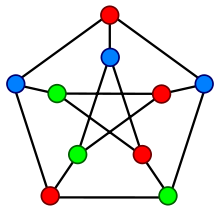
\includegraphics[width=\linewidth]{gcone.png} % Figure image
	\caption{A graph coloring example} % Figure caption
	\label{gcone} % Label for referencing with \ref{bear}
\end{figure}


\subsection{Maxinum Independent Set}
In graph theory, an independent set or stable set is a set of vertices in a
graph, no two of which are adjacent.
A maximal independent set (MIS) is an independent set
that is not a subset of any other independent set or equivalently can be defined
as that a maximal independent set is either an independent set such that adding
any other vertex to the set forces the set to contain an edge or the set of all vertices of the empty graph.
As Figure ~\ref{mistwo} suggested, for every two blue vertex, we can not find
such a edge to connect them. The MIS is the maxinum subset of graphs' all vertex who
satisfy the ruels. There are some clear rules for MIS.
\begin{itemize}
	\item the size of MIS for a forest is sum of size of MIS for every tree
    \item every sbuset except for empty set is still a independent set
	\item for a graph, there may be multiple different MIS, as suggested
        Figure ~\ref{misone}
\end{itemize}
To solve the MIS problem, almost immediately, a brute force method comes up with
us who's time complexity is O(\(2^n * n^2\)) for graph with n vertex. For every
sbuset of vertes sums up to \(2^n\) do a check to find out it's independent set
or not which need \(n^2\) steps. This algorithm is ediable just for a tiny graph
, dozens of vertex is the limitaion.

We can prove tha it's possible to reduce k-clique problem to MIS. If a graph
has a clique of size \textbf{k}, the inverse graph has an independent set of
size \textbf{k}. A clique of size \textbf{k} means that \textbf{k} nodes all
have edges in between them. In the inverse graph these \textbf{k} nodes are
not (directly) connected and can be used to create an independent set of size
\textbf{k}

\begin{figure}
	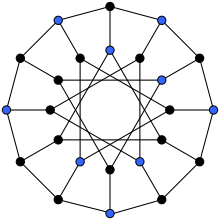
\includegraphics[width=\linewidth]{mistwo.png} % Figure image
	\caption{Bule vertex makes up a mis} % Figure caption
	\label{mistwo} % Label for referencing with \ref{bear}
\end{figure}

\begin{figure}
	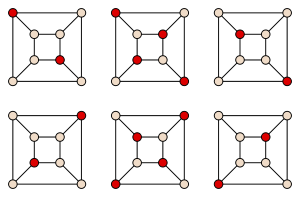
\includegraphics[width=\linewidth]{misone.png} % Figure image
	\caption{A graph whos mis is two} % Figure caption
	\label{misone} % Label for referencing with \ref{bear}
\end{figure}


%------------------------------------------------

\subsection{Operational Research}
As the complexity and specialization in an organization
increase, it becomes more and more difficult to allocate the available resources
to the various activities in a way that is most effective for the organization as a whole.
These kinds of problems and the need to find a better way to solve them provided
the environment for the emergence of \textbf{operations research} (commonly
referred to as \textbf{OR}).

MIS or graph coloring, they are all ask the same qustion, how to use the minimum
resources to meet the request. Many OR problems have strong background in
application, The major subdisciplines in modern operational research, as
identified by the journal Operations Research are:
\begin{itemize}
    \item Computing and information technologies
    \item Financial engineering
    \item Manufacturing, service sciences, and supply chain management
    \item Policy modeling and public sector work
    \item Revenue management
    \item Simulation
    \item Stochastic models
    \item Transportation
\end{itemize}

One way of summarizing the usual (overlapping) phases of an OR study is the following:
\begin{enumerate}
    \item Define the problem of interest and gather relevant data.
    \item Formulate a mathematical model to represent the problem.
    \item Develop a computer-based procedure for deriving solutions to the problem from the model.
    \item Test the model and refine it as needed.
    \item Prepare for the ongoing application of the model as prescribed by management.
    \item Implement.
\end{enumerate}



The Operational contains many branchs. In every branch, a bunch of methods have
developed for a cluster of similar questions.

An \textbf{integer programming} problem is a mathematical optimization or feasibility
program in which some or all of the variables are restricted to be integers. In
many settings the term refers to integer linear programming (ILP), in which the
objective function and the constraints (other than the integer constraints) are
linear.  Integer programming is NP-complete. In particular, the special case of
0-1 integer linear programming, in which unknowns are binary, and only the
restrictions must be satisfied, is one of Karp's 21 NP-complete problems.

In mathematics, \textbf{nonlinear programming} is the process of solving an optimization
problem defined by a system of equalities and inequalities, collectively termed
constraints, over a set of unknown real variables, along with an objective
function to be maximized or minimized, where some of the constraints or the
objective function are nonlinear.\citep{Reference13}

In computer science and \textbf{mathematical} optimization, a metaheuristic is a
higher-level procedure or heuristic designed to find, generate, or select a
heuristic (partial search algorithm) that may provide a sufficiently good
solution to an optimization problem, especially with incomplete or imperfect
information or limited computation capacity.\citep{Reference12}

\textbf{Game theory} \citep{Reference11} is "the study of mathematical models of conflict and cooperation
between intelligent rational decision-makers". Game theory is mainly used in
economics, political science, and psychology, as well as in logic and computer science

\textbf{Decision analysis}(DA) is the discipline comprising the philosophy, theory,
methodology, and professional practice necessary to address important decisions in a formal manner

\textbf{Queueing theory} \citep{Reference10}is the mathematical study of waiting lines, or queues.
A queueing model is constructed so that queue lengths and waiting time can be
predicted.\citep{Reference10} Queueing theory is generally considered a branch
of operations research because the results are often used when making business
decisions about the resources needed to provide a service.

\textbf{Inventory} theory, as it's name suggested, it studies the decisions faced by firms and
the military in connection with manufacturing, warehousing, supply chains, spare
part allocation and so on and provides the mathematical foundation for
logistics. The inventory control problem is the problem faced by a firm that
must decide how much to order in each time period to meet demand for its
products. The problem can be modeled using mathematical techniques of optimal
control, dynamic programming and network optimization. The study of such models
is part of inventory theory.

\subsection{Methods for Graph coloring}

Constructive greedy algorithm (\textbf{CGA}) is a type of heuristic
method which starts with an empty solution and repeatedly extends the current
solution until a complete solution is obtained. It differs from local search
heuristics which start with a complete solution and then try to improve the
current solution further via local moves. Examples of some constructive
heuristics developed for famous problems are: flow shop scheduling, vehicle
routing problem, open shop problem.

Genetic algorithm (\textbf{GA}) is a metaheuristic inspired by the process of natural
selection that belongs to the larger class of evolutionary algorithms (EA).
Genetic algorithms are commonly used to generate high-quality solutions to
optimization and search problems by relying on bio-inspired operators such as
mutation, crossover and selection.

Local search(\textbf{LC})is a heuristic method for solving computationally hard optimization
problems. Local search can be used on problems that can be formulated as finding
a solution maximizing a criterion among a number of candidate solutions. Local
search algorithms move from solution to solution in the space of candidate
solutions (the search space) by applying local changes, until a solution deemed
optimal is found or a time bound is elapsed.Figure \ref{intro} show a plain with
local minimization, it explained the same questions which local search will
encountered which can be avoided by tabu search in some degree by a special
techntechnology.
\begin{figure}
	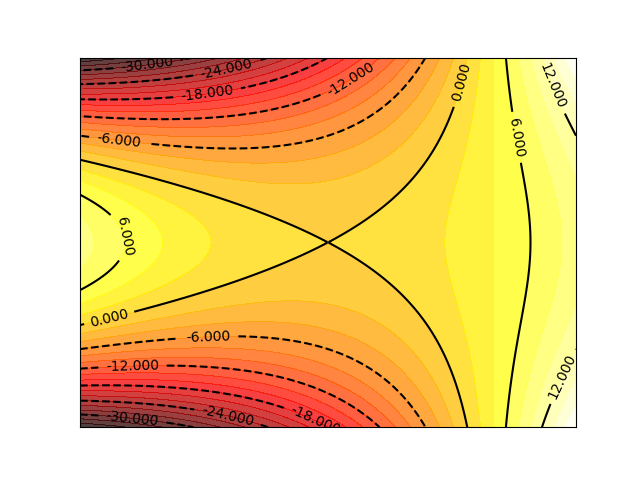
\includegraphics[width=\linewidth]{intro.png} % Figure image
	\caption{A with local minimization} % Figure caption
	\label{intro} % Label for referencing with \ref{bear}
\end{figure}


Successive building of color classes: This particular strategy consists in building successively
different color classes by identifying each time a maximal independent set and
removing its vertices from the graph. So the graph coloring problem is reduced to the
maximal independent set problem. Different techniques to find maximal independent sets
have been proposed for building successive color classes , including local
search methods . This strategy proves to be one of the most effective approaches
for coloring large random graphs.


\section{Tabu search}
Tabu search, created by Fred W. Glover in 1986 \citep{Reference5} and formalized
\citep{Reference6} \citep{Reference7} in 1989, is a metaheuristic search method
employing local search methods used for mathematical optimization.

Local (neighborhood) searches take a potential solution to a problem and check
its immediate neighbors (that is, solutions that are similar except for very few
minor details) in the hope of finding an improved solution. Local search methods
have a tendency to become stuck in suboptimal regions or on plateaus where many
solutions are equally fit.

Tabu search enhances the performance \citep{Reference8} of local search by relaxing its basic rule.
First, at each step worsening moves can be accepted if no improving move is
available(like when the search is stuck at a strict local minimum).
In addition, prohibitions (henceforth the term tabu) are introduced to
discourage the search from coming back to previously-visited solutions.

Here is the Pseudocode of general code:
\begin{lstlisting}
sBest <- s0
bestCandidate <- s0
tabuList <- []
tabuList.push(s0)
while (not stoppingCondition())
	sNeighborhood <- getNeighbors(bestCandidate)
	bestCandidate <- sNeighborHood.firstElement
	for (sCandidate in sNeighborHood)
		if ( (not tabuList.contains(sCandidate)) and (fitness(sCandidate) > fitness(bestCandidate)) )
			bestCandidate <- sCandidate
		end
	end
	if (fitness(bestCandidate) > fitness(sBest))
		sBest <- bestCandidate
	end
	tabuList.push(bestCandidate)
	if (tabuList.size > maxTabuSize)
		tabuList.removeFirst()
	end
end
return sBest
\end{lstlisting}

Beacuse the tabu algorithm is heuristic algorithm, here are some advice
\citep{Reference9} about how to make tabu search work better!

\begin{itemize}
    \item Tabu search was designed to manage an embedded hill climbing heuristic, although may be adapted to manage any neighborhood exploration heuristic.
    \item Tabu search was designed for, and has predominately been applied to discrete domains such as combinatorial optimization problems.
    \item Candidates for neighboring moves can be generated deterministically for the entire neighborhood or the neighborhood can be stochastically sampled to a fixed size, trading off efficiency for accuracy.
    \item Intermediate-term memory structures can be introduced (complementing the short-term memory) to focus the search on promising areas of the search space (intensification), called aspiration criteria.
    \item Long-term memory structures can be introduced (complementing the short-term memory) to encourage useful exploration of the broader search space, called diversification.
    \item Strategies may include generating solutions with rarely used components and biasing the generation away from the most commonly used solution components.
\end{itemize}

\subsection{Insight of Tabu Search}
As has been emphasized in the former section, the graph coloring algorithm can
a key to all kinds of the NP problems, the importance to understand and look
inside grapy coloring is wiseable to argue again.

For a optimization algorithm, one of the most tragdy things is losting the
courage to get out of the local oprimazation. Tabu algorithm, as it's name
suggested, it's key ideas forbits the algorithm stucking in the a pitch forever
by creating a forbiden list which document the latest steps leading to local
oprimazation and rejecting any attemptation to make such steps again. When doing
the business with the soruce code, how to maintain the tabu table efficiently
can be problem, as will be discussed later.

Figure~\ref{tabuone} shows a one possible instance to
color~\citep{Reference14} the graph, For current configuration, Table
~\ref{tabutable} shows the information about every node aspecting to how many
neighbors it has and how many conflicts exists.

\begin{figure}[h]
    \centering
    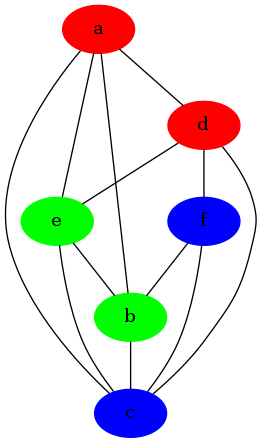
\includegraphics[width=0.25\textwidth]{tabuone.png}
    \caption{A instance of graph coloring}
    \label{tabuone}
\end{figure}

\begin{table}
	\caption{Example table}
	\centering
    \label{tabutable}
    \begin{tabular}{l*{3}{c}r}
        Vertex & color & Neighborhood & Conlict \\
    \hline
    a & red     &4 & 1   \\
    b & green   &4 & 1   \\
    c & blue    &5 & 1   \\
    d & red     &4 & 1   \\
    e & green   &4 & 1   \\
    f & blue    &3 & 1   \\
\end{tabular}
\end{table}
In order to reducing the total conflicts sperated in the whole graph, it's
naturally to design a algorithm which make a modication to a node's color which
can reducing conflicts. For example, if we exchange the color belonging to
\textbf{e} and \textbf{d}, the total conlicts will decrease one. Every time we
make such modification that will lead the conflicts decrease at the greatest
stride until we found the result or the times of iteration exceed the
limitaiton.

Tabu search illustrate a critical and creative idea to manipulate the procedure
of iteration, in order to jump out of the local minimal, modication resulting to
the increament of conflicts is preamble and manipulation on the same node is
forbiden to during a short time stride which is super paramter needed to be set
by our instinction. If the \textbf{tabu length} is set as \textbf{L}, in the
setp \textbf{a} the node M's color is changed , then during \textbf{a} and
\textbf{a + L}, the M is in the tabu status.

Here is a important aspiration for the tabu search, that is if one move can
override the best found solution found so far, it is accepted even if it is in
tabu status. The driven idea behind is alike that if you gain the best
performance ever by cheating, it's worthwhile to keep the record, if not, you
should give up the record for the sake of the risk brought with the cheeting.



\subsection{Pivotal technologies in implementation}
\begin{figure}[h]
    \centering
    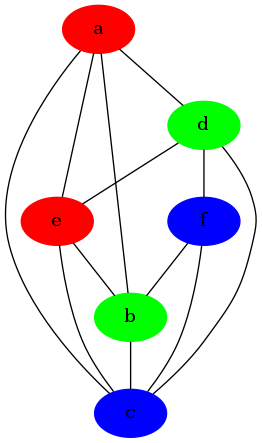
\includegraphics[width=0.25\textwidth]{tabutwo.png}
    \caption{A exchange of color}
    \label{tabutwo}
\end{figure}

\begin{table}
	\caption{Example table}
	\centering
    \label{tabutabletwo}
    \begin{tabular}{l*{3}{c}r}
        Vertex & color & Neighborhood & Conlict \\
    \hline
    a & red     &4 & 1   \\
    b & green   &4 & 0   \\
    c & blue    &5 & 1   \\
    d & red     &4 & 0   \\
    e & green   &4 & 1   \\
    f & blue    &3 & 1   \\
    \end{tabular}
\end{table}
If one node has been chosen to make a modification at step \textbf{a}, in the
next series steps, how to determine whether the node is in tabu status or not.
Many methods can be applied to this problem, for example, we can create a table
which keep a number for every node showing how many times before it can be
libertated from tabu status. Let's analyze this algorithm, assuming the tabu
length is \textbf{L}, we would at most have L nodes in the tabu status, we can
put these nodes in a red-black tree, every step, we should iterate from begin of
the tree to end to update every node's tabu status. So the time complexity is
O(\(\log{x}\) + L)

In fact, there is better way, determining whether a given node is in the tabu
status or not can be finished in O(1). First we create a timestamp table for
every node, then every time a node is updated for in the critical one move, we
set the node's timestamp at current step number, when we wanted to find out
whether the node is in the tabu status or not, we should check the difference
between current steps and the node's timestamp, if the difference is less than
than tabu length, then the node is in the tabu status.

\subsection{Implementation}
With key obstacle of tabu algorithm for graph coloring over comed, a clear and
particular description for the algorithm is necessary to convince the researcher
of superiority of tabu algorithm.

The base of the algorithm is some data structure essential in the runtime we
should initilize at the begining, as you can see, for the elegance and
algorithm, there are merely few data structures should maintained during the
code runging. \textbf{tabu\_tenure} is used for determining the node's tabu
status efficiently, \textbf{adjacent\_color\_table} is used for recording
neighbors's colors, \textbf{solutions} is used for recording the every nodes'
color. \textbf{conflict\_num} is used for finding out the best result already get
, if the conflict\_num is equal to zero, then the result is found and should
stop. Maybe for some super paramter, the algorithm will never stop, the
\textbf{max\_iter} is used to shut it down when iterate too many times.

\begin{lstlisting}
    // runtime data
    std::vector<unsigned int> solutions;
    std::vector<std::vector<unsigned int> > tabu_tenure;
    std::vector<std::vector<unsigned int> > adjacent_color_table;
    int conflict_num;
\end{lstlisting}

the kernel idea of tabu search for graph coloring is keep \textbf{find\_move}
and \textbf{make\_move} until the number of conflits reduced to zero or
iteration times meet the limitaion.\textbf{make\_move} is fairly simple enough
to omited, but \textbf{find\_move} contains the main ideas of the tabu search.
The cpp code is given as below. For every node and for every color, calculated
the conflict reduction by a critical one move. At last, make a aspiration test.

\begin{lstlisting}
void Tabu::find_move(TabuMove& tabu_move, unsigned int iter){
TabuMove tabu_best_move;
TabuMove non_tabu_best_move;

for(int i = 1; i <= N; i++){

if(adjacent_color_table[i][solutions[i]] != 0){

for(int k = 0; k < K; k++){

if(k == solutions[i]) continue;

int delta = (int)adjacent_color_table[i][k] -
    (int)adjacent_color_table[i][solutions[i]];


if(iter < tabu_tenure[i][k]){
if(delta < tabu_best_move.delta)
tabu_best_move = TabuMove(i, solutions[i], k, delta);
}else{
if(delta < non_tabu_best_move.delta)
non_tabu_best_move = TabuMove(i, solutions[i], k, delta);
} } } }


bool is_aspiration =
    (tabu_best_move.delta < 0 && non_tabu_best_move.delta > 0);
if(is_aspiration)
    tabu_move = tabu_best_move;
else
    tabu_move = non_tabu_best_move;
}
\end{lstlisting}

\subsection{Analysis of the experiments}

Before analysis of the experiments, carefully experimentation is needed as a
strong stepping stone. As for tabu search, some super parameters are required to
tuning.
\begin{itemize}
	\item Maxinum Iteration num
	\item Tabu length
    \item Color Nums
\end{itemize}



In the Tabele \ref{tabu:res}, it's clear that different \textbf{color num} and
\textbf{tabu lengtha} are tested with different data base and corresponding
\textbf{iteration num} and \textbf{time}. In this experiment, we use the data
came from the same source \citep{Reference1}.

In the Table \ref{hea:res}, for the reason that the textline width can not hold
the whole table and personal aesthetic demanding, the table column name is
abbreviated. Here is the explanation.


\begin{description}
	\item[SN] series number, begin at 1 and increase one by one
    \item[D] data source, the data used to test the algorithm
    \item[TL] tabu length, a super parameter to decide how long the tabu status
        last when a node is modified
    \item [T] time, the time program takes to finish, if it can not find the
        result, the time will be set as null, the time is measured by seconds.
    \item [CN] color numbers, the color numbers for the program to construct a
        graph coloring result.
\end{description}

\begin{table}
	\caption{Tabu Search Experiment Results}
	\centering
    \label{tabu:res}
    \begin{tabular}{l*{4}{c}r | p{1cm}}
        SN & D & CN & T & TL  \\
    \hline
    1 & DSJC125.1 &5 &   0.013845 & 10     \\
    2 & DSJC250.1 &8 &   0.252603 & 10    \\
    3 & DSJC250.5 &28 & 95.3894   & 10     \\
    4 & DSJC250.9 &72 & NULL   & 10    \\
    5 & DSJC500.1 &13 & 0.187932   & 10    \\
    6 & DSJC500.1 &12 & NULL   & 10    \\
    7 & DSJC250.9 &73 &  NULL  & 10    \\
    8 & DSJC250.9 &100 &  0.055752  & 10    \\
    8 & DSJC250.9 &75 &  NULL  & 10    \\
    9 & DSJC250.9 &80 &  0.115334  & 10    \\
    10 & DSJC500.5 &51 & 6.62945   & 10    \\
    11 & DSJC500.5 &50 & 251.354   & 10    \\
    12 & DSJC500.5 &49 & NULL   & 10    \\
    13 & DSJC1000.1 &22 & 0.920005   & 10    \\
    14 & DSJC1000.1 &25 & 0.020005   & 10    \\
    15 & DSJC1000.1 &21 & 36.9668   & 10    \\
    \end{tabular}
\end{table}

How to represent the graph is so important although there are multiple ways to
implement is, the most common one is adjacent list, many coders are also
familiar with adjacent table which is not so friendly to computing resource and
memory. In fact, there is third way to represent the table called forward list,
which is required the number of edges before establishing the data structure.
All in all, adjacent list and forward list make little difference when the
mainly costage arised from tabu search



\section{Hybrid Evolutionary Algorithm}
Hybrid Evolutionary Algorithms(\textbf(HEA)) is powerful Graph Coloring \citep{Galinier1999}
based on tabu search. HEAs can  applied to some well-known NP-hard combinatorial
problems such as the traveling salesman problem, the quadratic assignment
problem and the bin-packing problem.  The results obtained by HEA support the
the perspective that it's another powerful and sharp sword to confront the
complexity of NP program.

Hybrid evolutionary algorithm has a relatively stringent restriction of cross
over operation, that's saying the designing the cross over operation is the
central assignment of developing this algorithm.

As one of important heuristic algorithms, hybrid algorithm use a another
technology called cross over to make algorithm more diversity.

Figure \ref{heaone} shows the general procedures HEA process.

\begin{figure}
	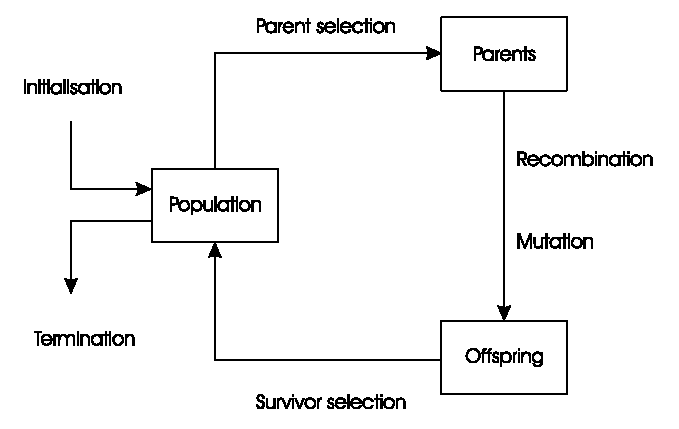
\includegraphics[width=\linewidth]{HEAone.png} % Figure image
	\caption{Procedure of HEA!} % Figure caption
	\label{heaone} % Label for referencing with \ref{bear}
\end{figure}

\subsection{Algorithm Description}

Hybrid evolutionary algorithm is based on the tabu search, but the key part is
the crossover operation. Apart from cross over, there are still some point
needed to discuss carefully. First of all, the size of population is a really
important super parameter when running the code, during the experiments, strong
evidence proved that with popultaion increasing, the difficulty to find the
corrrect result surges.

Modest modification for the tabu search is needed too. We should add two
variable, \textbf{min\_conflict\_num} and \textbf{best\_solution} to the tabu
search code, for the purpose that the best result during tabu search is
indivisible for later analysis.

Crossover is easy to implemented, but it's not easy to understand the idea
inside it, first at all, we have proved before that a legal coloring coloring
with k different kings of color is a collection of k independent sets. So if we
can find the maxinum independent set, it's going to make it to get a valid k
coloring schema.In other words, the more vertices are transmitted from parent
individuals to the offspring within k steps, the less vertices are
left unassigned.In this way, the obtained offspring individual has more
possibility to become a legal coloring.

In order to create populaiton, we should define a class to save every tabu
search result for later usage, it contains two elements, the one is
\textbf{conflict\_num} and the other one is \textbf{solution}. We create a array
of Tabu search result, and random choose two of them, by doing crossover, a new
result generated, accroding to the result of experiment, the new generated
result just keep a good structure and fail to give a grade aspecting to
conflicts, so tabu search is needed for the new generated resutl. As you can
see, two slightly different version Tabu search is required.

\pagebreak
\subsection{Implementation}

Two main parts are added on the base of Tabu search, crossover and main loop.

The pseudocode code of corssover is listed as follow, configuration \textbf{c1}
and \textbf{c2} are choosed randomly from population, then find the set of
biggest cardinality from c1 and c2 in turn, every time a set is chooed out of
the configuration, all the elements of if should be removed from the two
configurations totally. There is a high possibility that even the loop ends,
there are still some vertex not allocated, the strategy is random distributing
the remaining vertex. The cpp code needs to deal with many disgusting details,
making it not wiseable to print it here, so they are neglected.

\begin{lstlisting}
Data : configuration = c1 configuration = c2; color_number = K
for i in range(K):
    if i is odd
        choose the most cardinality set s of c1
        remove the elements of s from c1 and c2
    else
        choose the most cardinality set s of c2
        remove all elements of s from c1 and c2
Assign the result vertices randomly
\end{lstlisting}

The main loop started with making several Tabu search whoes result making up a
popultaion used for later crossover. The keep doing the loop. The loop contains
the following procedures:
\begin{enumerate}
    \item choose the parents
    \item do crossover based on the parents
    \item do tabu search with the crossover result
    \item weed out the worst individual in the populaiton
\end{enumerate}
Some superparameter is needed, for example, \textbf{populaiton size}
\textbf{tabu search maxinum iteration tims} should be carefully designed to get
good result.

There is small trick when tuning the super parameters, because of the fact that
evolution base on a mount of populaiton and it's time consuming to generate the
populaiton, we can save the population to disk, then every time we needed use
it, just loaded it.


\subsection{Analyzation of the Results}

The result is contained in the table  \ref{HEA:res}, the data source
\citep{Reference1}is same. From the result, at least two conclusion we can
get, for some data, HEA can do bette, although it needs to generate population,
which is great cost. The Second, the HEA can achieve better result, which is
rather important.
For the same reason, abbreviation is used.
\begin{description}
	\item[IN] index, begin at 1 and increase one by one
	\item[PS] index, begin at 1 and increase one by one
\end{description}

\begin{table}
	\caption{HEA Search Experiment Results}
	\centering
    \label{HEA:res}
    \begin{tabular}{l*{4}{c}r | p{1cm}}
        IN & D & CN & T & TL & PS  \\
    \hline
    1 & DSJC125.1 &5 &  0.063239  & 10 & 5    \\
    2 & DSJC250.1 &8 &   0.723432 & 10 & 5    \\
    3 & DSJC500.5 &52 &  10.3452  & 10 & 5    \\
    4 & DSJC500.5 &51 &  33.7604  & 10 & 5    \\
    5 & DSJC500.5 &50 & 109.607  & 10 & 5    \\
    5 & DSJC500.5 &49 & NULL  & 10 & 4    \\
    5 & DSJC500.5 &49 & NULL  & 10 & 10    \\
    6 & DSJC1000.1 &25 & 1.69291  & 10 & 5    \\
    \end{tabular}
\end{table}

In fact, the evidence is kind of discouraging, because the leap from tabu search
to HEA is smaller than what we expected.


\section{Summarize}

\subsection{Inspiration and Review}
Although graph coloring is NP problem, many creative algorithm belonging to
\textbf{OR} can achieve good result with acceptable time consuming and computing
resources demanding. Two representative approaches, Tabu search and Hybrid
Evolutionary, as described above proves that heuristic algorithm is sharp
precise arrow to the target.During the experiment, the super parameters occupy
the decisive position of the experiment results, this drawback is a common
drawbakc for almost all algorithms related to heuristics. Even if good suer
paramters can be detected by the tremendous efforts and innumerable attempts,
the results primarily dominated by the algorithm itself. Indulging in tuning the
super parameters detrimental to creativeness and liver.

Another important factor of the implementation is optimization of the iteration.
The times of iteration almost reaches to million, that means a unobervable
reduction of time comsuming in one iteration leads to a huge efficiency
promotion. As for how to optimize the iteration, many pragmatic and available
trick can be applied. As for language, C and Cpp is preferred, for the sake of
taking advantage of their peculiarity in hardware utilization.  Understanding
some basic knowledge about compiler and computer system also is of great
signification, locality principal guide the coder to utilize computers' cache
completely, being familiar with complier can avoid some drawback and limitaiton
of compiler.

\subsection{Suggestion about course}
It's not a blandishment for me to appraise this course as a milestone in my
own undergraduate learning tutorial. For the past three years, everyone is
talking about algorithm with me, but in fact, our discussion is limited to the
P program which can be addressed in the polynomial time. All kinds of on line
judge and endless interview question summarizing keep inducing us to believe
that once specialize in the P problem, we can cope with any quesiton. But
\textbf{Operational Research} give us a hidden side long neglected by so called
algorithm textbook, this side we call algorithm in application. The famous
algorithm \textbf{Introduction of Algorithm} shows many fundamental algorithm
useful in almost every programming project, but we should admit that these
algorithm is too abstract and high level, which is not suitable for a
concrete project, \textbf{OR} is a great supplement for that. When we are facing
the a complex problem in application, when we are at a loss after finding that
the qucik sort algorithm can not cover the requirment of the quesiton at hand,
referring to the operational research is sagacious.

In a department which is almost totally controlled by the computer system group
and wuhan national laboratory of optoelectronics, every course about algorithm,
operation system, computer network is being squeezed out by cutting downing
course hours or degregrating the quality. For us, every course irrelevant with
hardware is precise enough to enjoy,

After skipping some operational research books, I do feel disappointed about
what I have learn. When taking the course, implementing the algorithm what we
learned  and writing this report, I feel like doing a project with old knowledge
rather than by a new idea or technology. In another word, what I learn is much
lesser than I expected. Maybe the consequenc is resutled from short course hours
and a huge classroom and mingled students.

All in all, this course shed a new aspect about algorithm to me ! Thanks
everyone devoted to the course !



%----------------------------------------------------------------------------------------
%	BIBLIOGRAPHY
%----------------------------------------------------------------------------------------

\pagebreak
\printbibliography[title={Bibliography}] % Print the bibliography, section title in curly brackets

\newcommand\blankpage{%
    \null
    \thispagestyle{empty}%
    \addtocounter{page}{-1}%
    \newpage}
%----------------------------------------------------------------------------------------


\end{document}
